\documentclass[aspectratio=169,11pt]{beamer}
\usetheme{default}
\setbeamertemplate{navigation symbols}{}
\setbeamertemplate{footline}{%
  \hfill\insertframenumber/\inserttotalframenumber\hspace*{4pt}\vspace{2pt}%
}
\usepackage{lmodern}
\usepackage[most]{tcolorbox}
\usepackage{listings}
\usepackage{tikz}
\usetikzlibrary{arrows.meta,positioning,shapes.geometric,fit,backgrounds}
\usepackage{booktabs}
\usepackage{hyperref}

\definecolor{lcgreen}{HTML}{2E7D32}
\definecolor{lcblue}{HTML}{1565C0}
\definecolor{lcorange}{HTML}{EF6C00}
\definecolor{lcred}{HTML}{C62828}
\definecolor{codebg}{HTML}{F5F5F5}
\definecolor{docgray}{gray}{0.55}

\newtcolorbox{conceptbox}[1][]{colback=yellow!20,colframe=yellow!60!black,title=#1,fonttitle=\bfseries,top=2pt,bottom=2pt,left=4pt,right=4pt}
\newtcolorbox{warningbox}[1][]{colback=red!15,colframe=red!60!black,title=#1,fonttitle=\bfseries,top=2pt,bottom=2pt,left=4pt,right=4pt}
\newtcolorbox{tipbox}[1][]{colback=green!10,colframe=green!50!black,title=#1,fonttitle=\bfseries,top=2pt,bottom=2pt,left=4pt,right=4pt}
\newtcolorbox{codebox}[1][]{colback=blue!10,colframe=blue!40!black,title=#1,fonttitle=\bfseries,top=2pt,bottom=2pt,left=4pt,right=4pt}

\lstset{
  basicstyle=\ttfamily\tiny,
  backgroundcolor=\color{codebg},
  breaklines=true,
  frame=single,
  rulecolor=\color{blue!40!black},
  keywordstyle=\color{lcblue}\bfseries,
  stringstyle=\color{lcgreen},
  commentstyle=\color{docgray}\itshape,
  language=Python,
  showstringspaces=false,
  tabsize=2,
  xleftmargin=2pt,
  xrightmargin=2pt,
  aboveskip=2pt,
  belowskip=2pt,
}

\newcommand{\docref}[1]{{\scriptsize\color{docgray}[Docs: #1]}}

\title{LangChain: Runnables \& LCEL}
\subtitle{LangChain Expression Language for Composable AI Systems}
\author{Section 03 \texttt{langchain-core v1.2.x}}
\date{March 2026}

\begin{document}

% =============================================================================
% TITLE SLIDE
% =============================================================================
\begin{frame}
  \titlepage
  \vspace{0.3em}
  \begin{center}
    {\color{lcblue}\textbf{Building composable, type-safe AI applications with LCEL}}
  \end{center}
\end{frame}

% =============================================================================
% AGENDA
% =============================================================================
\begin{frame}{Agenda}
  \begin{itemize}\setlength{\itemsep}{1pt}
    \item \textbf{What is LCEL?} The mental model
    \item \textbf{The Runnable protocol} — invoke, batch, stream, async variants
    \item \textbf{The pipe operator} |  — composition syntax
    \item \textbf{Building chains} — prompt | model | parser
    \item \textbf{Data flow patterns} — Passthrough, Parallel, Lambda, Branch
    \item \textbf{Resilience} — fallbacks, retries, configuration
    \item \textbf{Advanced patterns} — complex chains, debugging, performance
    \item \textbf{Comparison} — LCEL vs legacy Chain classes
    \item \textbf{Cheat sheet \& self-check}
  \end{itemize}
  \vspace{0.3em}
  \small \textit{Coverage: LangChain v1.2.x (Core + Community packages)}
\end{frame}

% =============================================================================
% SECTION 1: MENTAL MODEL
% =============================================================================
\section{Mental Model: LCEL as Composition}

\begin{frame}{What is LCEL?}
  \textbf{LCEL = LangChain Expression Language}

  \vspace{0.3em}
  \begin{conceptbox}[Definition]
    A declarative API for composing language model applications into modular,
    reusable, and type-safe data pipelines using a consistent \textbf{Runnable protocol}.
  \end{conceptbox}

  \vspace{0.3em}
  \textbf{Three pillars:}
  \begin{enumerate}\setlength{\itemsep}{1pt}
    \item \textbf{Runnable Protocol} — standardized interface for any component
    \item \textbf{Pipe Operator} | — chainable, readable syntax
    \item \textbf{Type Safety} — input/output schemas ensure compatibility
  \end{enumerate}

  \vspace{0.3em}
  \textit{Think: Unix pipes, but for LLM workflows.}
\end{frame}

\begin{frame}{Why LCEL? The Problem}
  \textbf{Legacy Chain classes had pain points:}

  \begin{itemize}\setlength{\itemsep}{1pt}
    \item Different `.run()` / `.call()` signatures across chain types
    \item No standard way to compose chains together
    \item Async support was inconsistent (or missing)
    \item Streaming didn't work reliably
    \item Type hints were weak; runtime errors common
    \item Hard to test, debug, and reuse components
  \end{itemize}

  \vspace{0.3em}
  \textbf{LCEL solves this:}

  \begin{itemize}\setlength{\itemsep}{1pt}
    \item One protocol, one syntax, unlimited flexibility
    \item Compose anything into anything (prompt + model + parser)
    \item First-class async and streaming
    \item Input/output schemas define contracts
    \item Easy to test, debug, and share
  \end{itemize}
\end{frame}

\begin{frame}{The Unix Philosophy Applied to LLMs}
  \begin{center}
    \texttt{\$ echo "What is gravity?" | curl-llm | json-parser}
  \end{center}

  \vspace{0.3em}
  \small
  \begin{tabular}{ll}
    \textbf{Unix pipe} & \textbf{LCEL equivalent} \\
    \hline
    \texttt{echo} (text source) & Prompt, input dict \\
    \texttt{|} (pipe) & \texttt{|} (same syntax!) \\
    \texttt{curl-llm} (process) & LLM, custom Runnable \\
    \texttt{json-parser} (transform) & Parser, RunnableLambda \\
  \end{tabular}

  \vspace{0.3em}
  \small \textit{The mental model: data flows left-to-right; each stage transforms and passes to the next.}
\end{frame}

% =============================================================================
% SECTION 2: THE RUNNABLE PROTOCOL
% =============================================================================
\section{The Runnable Protocol}

\begin{frame}{Runnable: The Universal Interface}
  \begin{codebox}[Core Methods]
\begin{lstlisting}
# Synchronous methods
.invoke(input) -> output
.batch(inputs: List) -> List[output]
.stream(input) -> Iterator[output]

# Asynchronous methods
async .ainvoke(input) -> output
async .abatch(inputs: List) -> List[output]
async .astream(input) -> AsyncIterator[output]
\end{lstlisting}
  \end{codebox}

  \vspace{0.12em}
  \textbf{Key idea:} Every LangChain component implements this protocol.

  \begin{itemize}\setlength{\itemsep}{1pt}
    \item LLMs, prompts, parsers, retrievers, tools, custom functions
    \item All composable; all have the same interface
    \item Mix sync/async freely (LCEL handles the plumbing)
  \end{itemize}
\end{frame}

\begin{frame}[fragile]{Runnable Protocol: Sync & Async}
  \begin{codebox}[Example: Prompt + LLM]
\begin{lstlisting}
from langchain_core.prompts import ChatPromptTemplate
from langchain_openai import ChatOpenAI

prompt = ChatPromptTemplate.from_template(
    "Explain {topic} in 2 sentences."
)
model = ChatOpenAI(model="gpt-4")
chain = prompt | model

# Sync: invoke returns one output
output = chain.invoke({"topic": "gravity"})

# Batch: invoke multiple inputs
outputs = chain.batch(
    [{"topic": "gravity"}, {"topic": "light"}]
)

# Async: handle thousands concurrently
output = await chain.ainvoke({"topic": "gravity"})
\end{lstlisting}
  \end{codebox}
\end{frame}

\begin{frame}[fragile]{Streaming: Real-time Token Output}
  \begin{codebox}[Streaming with .stream()]
\begin{lstlisting}
# Synchronous streaming (print tokens as they arrive)
for chunk in chain.stream({"topic": "quantum physics"}):
    print(chunk.content, end="", flush=True)

# Async streaming (for web apps, async servers)
async for chunk in chain.astream({"topic": "quantum physics"}):
    print(chunk.content, end="", flush=True)

# Batch + stream: process multiple inputs with progress
for output in chain.batch([...], {max_concurrency: 5}):
    # Each output is fully streamed before next starts
    print(output)
\end{lstlisting}
  \end{codebox}

  \vspace{0.12em}
  \small \textit{Streaming is critical for user-facing LLM apps (show tokens as they're generated, not all at once).}
\end{frame}

\begin{frame}{When to Use Each Method}
  \begin{tabular}{|l|l|l|}
    \hline
    \textbf{Method} & \textbf{Use case} & \textbf{Example} \\
    \hline
    \texttt{invoke()} & Single input, wait for response & API endpoint \\
    \hline
    \texttt{batch()} & Many inputs, maximize throughput & Processing dataset \\
    \hline
    \texttt{stream()} & Single input, show tokens live & Chat UI, notebooks \\
    \hline
    \texttt{ainvoke()} & Async web app, non-blocking & FastAPI endpoint \\
    \hline
    \texttt{abatch()} & Async, many inputs & Async worker pool \\
    \hline
    \texttt{astream()} & Async, live tokens & WebSocket chat \\
    \hline
  \end{tabular}

  \vspace{0.3em}
  \small \textbf{Rule of thumb:} Use \texttt{batch()} for throughput, \texttt{stream()} for UX, \texttt{async} for scalability.
\end{frame}

% =============================================================================
% SECTION 3: THE PIPE OPERATOR
% =============================================================================
\section{The Pipe Operator}

\begin{frame}[fragile]{The Pipe Operator: Syntax \& Semantics}
  \begin{codebox}[Pipe Composability]
\begin{lstlisting}
# Pipe operator: a | b creates a RunnableSequence
# Data flows: a.invoke(input) -> b.invoke(result)

chain = prompt | model | output_parser

# Equivalent to:
# Step 1: prompt.invoke({"topic": "..."})
#   -> PromptValue
# Step 2: model.invoke(PromptValue)
#   -> AIMessage(content="...")
# Step 3: output_parser.invoke(AIMessage)
#   -> Parsed output (str, dict, object)
\end{lstlisting}
  \end{codebox}

  \vspace{0.12em}
  \begin{tipbox}[Key Insight]
    The pipe operator is \textbf{syntactic sugar}. Under the hood, it creates a
    \texttt{RunnableSequence} that orchestrates the flow.
  \end{tipbox}
\end{frame}

\begin{frame}[fragile]{Pipe Operator: How It Works}
  \begin{codebox}[Under the Hood]
\begin{lstlisting}
from langchain_core.runnables import RunnableSequence

# These are equivalent:
chain1 = prompt | model | parser

chain2 = RunnableSequence(
    first=RunnableSequence(
        first=prompt,
        last=model
    ),
    last=parser
)

# Both have .invoke(), .stream(), .batch(), etc.
output1 = chain1.invoke({"topic": "gravity"})
output2 = chain2.invoke({"topic": "gravity"})
# output1 == output2
\end{lstlisting}
  \end{codebox}

  \vspace{0.12em}
  \small The pipe operator nests automatically; LCEL handles intermediate steps.
\end{frame}

\begin{frame}[fragile]{Pipe: More Than Sequence}
  \begin{codebox}[Pipe with Operators]
\begin{lstlisting}
# Pipe + dict shorthand creates RunnableParallel
parallel_chain = {
    "question": RunnablePassthrough(),
    "context": retriever
} | prompt | model

# Pipe + conditional creates RunnableBranch
branch_chain = (
    condition_runnable
    | {
        "path_a": chain_a,
        "path_b": chain_b
    }
)

# Pipe + add creates RunnableSequence with assignment
chain = prompt | model | {"original": RunnablePassthrough(), "parsed": parser}
\end{lstlisting}
  \end{codebox}

  \vspace{0.12em}
  \small The pipe operator is polymorphic: dict means parallel, list means branching, Runnable means sequential.
\end{frame}

% =============================================================================
% SECTION 4: BUILDING YOUR FIRST CHAIN
% =============================================================================
\section{Building Your First Chain}

\begin{frame}[fragile]{The Classic Pattern: Prompt | Model | Parser}
  \begin{codebox}[Complete Example]
\begin{lstlisting}
from langchain_core.prompts import ChatPromptTemplate
from langchain_openai import ChatOpenAI
from langchain_core.output_parsers import StrOutputParser

# 1. Define prompt template
prompt = ChatPromptTemplate.from_template(
    "Explain {topic} in 2 sentences."
)

# 2. Choose LLM
model = ChatOpenAI(model="gpt-4", temperature=0.7)

# 3. Add parser
parser = StrOutputParser()

# 4. Compose
chain = prompt | model | parser

# 5. Run
result = chain.invoke({"topic": "machine learning"})
print(result)  # "Machine learning is..."
\end{lstlisting}
  \end{codebox}

  \docref{https://python.langchain.com/docs/expression\_language}
\end{frame}

\begin{frame}[fragile]{Input/Output Schemas}
  \begin{codebox}[Schema Inspection]
\begin{lstlisting}
# Every Runnable has input_schema and output_schema
chain = prompt | model | parser

print(chain.input_schema.schema())
# {
#   "type": "object",
#   "properties": {
#     "topic": {"type": "string"}
#   }
# }

print(chain.output_schema.schema())
# {"type": "string"}

# Schemas enable:
# - Type checking before runtime
# - Auto-documentation
# - Request validation in APIs
# - IDE autocompletion
\end{lstlisting}
  \end{codebox}

  \vspace{0.12em}
  \small \textit{Input/output schemas are the contract: they define what the Runnable accepts and produces.}
\end{frame}

\begin{frame}[fragile]{Real-world: RAG Chain}
  \begin{codebox}[Retrieval-Augmented Generation]
\begin{lstlisting}
from langchain.vectorstores import Chroma
from langchain_core.runnables import RunnablePassthrough

# 1. Retriever
retriever = Chroma.from_documents(...).as_retriever()

# 2. Prompt with context placeholder
prompt = ChatPromptTemplate.from_template("""
    Answer based on context:
    Context: {context}
    Question: {question}
""")

# 3. Format: pass through Q, retrieve context
chain = (
    {"context": retriever, "question": RunnablePassthrough()}
    | prompt
    | model
    | StrOutputParser()
)

# 4. Run with just the question
answer = chain.invoke("What is RAG?")
\end{lstlisting}
  \end{codebox}
\end{frame}

% =============================================================================
% SECTION 5: RUNNABLEPASSTHROUGH
% =============================================================================
\section{Data Flow Patterns}

\begin{frame}[fragile]{RunnablePassthrough: Identity Transformation}
  \begin{codebox}[Passing Data Through]
\begin{lstlisting}
from langchain_core.runnables import RunnablePassthrough

# Identity: returns input unchanged
passthrough = RunnablePassthrough()
output = passthrough.invoke("hello")
# output == "hello"

# In a chain: used with dict to keep input available
chain = (
    {"input": RunnablePassthrough(), "output": model}
    | format_results_template
)

# With .assign(): add computed fields without losing input
chain = (
    {"input": RunnablePassthrough()}
    | RunnablePassthrough.assign(
        computed=lambda x: len(x["input"].split())
    )
)
# Returns: {"input": "...", "computed": 5}
\end{lstlisting}
  \end{codebox}

  \docref{RunnablePassthrough}
\end{frame}

\begin{frame}[fragile]{RunnableParallel: Multiple Branches}
  \begin{codebox}[Running Tasks in Parallel]
\begin{lstlisting}
from langchain_core.runnables import RunnableParallel

# Dict shorthand automatically creates RunnableParallel
parallel = {
    "question": RunnablePassthrough(),
    "length": RunnableLambda(lambda x: len(x)),
    "upper": RunnableLambda(lambda x: x.upper())
}

result = parallel.invoke("hello")
# {
#   "question": "hello",
#   "length": 5,
#   "upper": "HELLO"
# }

# Explicitly: RunnableParallel(...)
explicit = RunnableParallel(
    question=RunnablePassthrough(),
    length=RunnableLambda(len)
)

# All branches execute in parallel; combine results
\end{lstlisting}
  \end{codebox}

  \docref{RunnableParallel}
\end{frame}

\begin{frame}[fragile]{RunnableLambda: Wrapping Python Functions}
  \begin{codebox}[Converting Functions to Runnables]
\begin{lstlisting}
from langchain_core.runnables import RunnableLambda

# Wrap a function as a Runnable
def uppercase(x):
    return x.upper()

runnable = RunnableLambda(uppercase)
output = runnable.invoke("hello")
# "HELLO"

# Async functions too
async def fetch_data(topic):
    # await expensive_api_call(topic)
    return f"Data for {topic}"

async_runnable = RunnableLambda(fetch_data)
output = await async_runnable.ainvoke("AI")

# In chains: seamless composition
chain = prompt | model | RunnableLambda(lambda x: x.upper())
\end{lstlisting}
  \end{codebox}

  \docref{RunnableLambda}
\end{frame}

\begin{frame}[fragile]{RunnableSequence: Explicit Composition}
  \begin{codebox}[Explicitly Composed Sequences]
\begin{lstlisting}
from langchain_core.runnables import RunnableSequence

# The pipe operator creates RunnableSequence
chain1 = prompt | model | parser

# Explicit construction
chain2 = RunnableSequence(
    steps=[prompt, model, parser]
)

# Both are equivalent
output1 = chain1.invoke({"topic": "AI"})
output2 = chain2.invoke({"topic": "AI"})

# Access individual steps
for i, step in enumerate(chain2.steps):
    print(f"Step {i}: {step}")

# Debug: see intermediate outputs
# (Use .stream() to see step-by-step execution)
\end{lstlisting}
  \end{codebox}

  \small Most of the time, use pipe; RunnableSequence is for programmatic construction.
\end{frame}

% =============================================================================
% SECTION 6: BRANCHING & CONDITIONAL LOGIC
% =============================================================================

\begin{frame}[fragile]{RunnableBranch: Conditional Routing}
  \begin{codebox}[If-Then-Else Logic]
\begin{lstlisting}
from langchain_core.runnables import RunnableBranch

# Create conditions and routes
branches = RunnableBranch(
    (lambda x: "python" in x.lower(), python_chain),
    (lambda x: "javascript" in x.lower(), js_chain),
    default_chain  # fallback
)

# Or with RunnableBranch.route_on_type() helper
from langchain_core.messages import AIMessage, HumanMessage

branches = RunnableBranch(
    (lambda x: isinstance(x, HumanMessage), human_handler),
    (lambda x: isinstance(x, AIMessage), ai_handler),
    unknown_handler
)

# Invoke
output = branches.invoke("Show me Python code")
# Routes to python_chain
\end{lstlisting}
  \end{codebox}

  \docref{RunnableBranch}
\end{frame}

\begin{frame}[fragile]{Branching: Complex Patterns}
  \begin{codebox}[Multi-Level Routing]
\begin{lstlisting}
# Dynamically choose chain based on input
def route_model(question):
    if "quantum" in question.lower():
        return "chain_for_physics"
    elif "biology" in question.lower():
        return "chain_for_biology"
    return "default_chain"

# Combined with pipe
chain = (
    {"question": RunnablePassthrough()}
    | RunnableBranch(
        (lambda x: "quantum" in x["question"].lower(), physics_chain),
        (lambda x: "biology" in x["question"].lower(), bio_chain),
        RunnableLambda(lambda x: general_chain.invoke(x["question"]))
    )
)

output = chain.invoke("What is quantum entanglement?")
# Routes to physics_chain
\end{lstlisting}
  \end{codebox}
\end{frame}

% =============================================================================
% SECTION 7: RESILIENCE PATTERNS
% =============================================================================
\section{Resilience \& Configuration}

\begin{frame}[fragile,shrink=3]{Fallbacks: Graceful Degradation}
  \begin{codebox}[Fallback Chains]
\begin{lstlisting}
from langchain_core.runnables import RunnableLambda

# Primary chain
primary = prompt | model

# Fallback chain (e.g., cheaper model or API)
fallback = prompt | ChatOpenAI(model="gpt-3.5-turbo")

# Combine with .with_fallbacks()
chain = primary.with_fallbacks([fallback])

# If primary fails (timeout, error), try fallback
output = chain.invoke({"topic": "AI"})

# Multiple fallbacks: try in order
chain = (
    primary
    .with_fallbacks([fallback1, fallback2, fallback3])
)

# Configure exception types to catch
chain = primary.with_fallbacks(
    [fallback],
    exceptions_to_handle=(TimeoutError, ValueError)
)
\end{lstlisting}
  \end{codebox}

  \docref{with\_fallbacks}
\end{frame}

\begin{frame}[fragile,shrink=3]{Retry Logic: Resilience}
  \begin{codebox}[Automatic Retries]
\begin{lstlisting}
# Retry with exponential backoff
chain = (
    prompt | model
).with_retry(
    stop=stop_after_attempt(3),
    wait=wait_exponential(multiplier=1, min=1, max=10),
    retry=retry_if_exception_type(RateLimitError)
)

# Or use tenacity directly
from tenacity import retry, stop_after_attempt, wait_exponential

@retry(stop=stop_after_attempt(3))
def call_chain(input_data):
    return chain.invoke(input_data)

# Retry on specific exceptions
chain = (
    prompt | model
).with_retry(
    retry=retry_if_exception_type((TimeoutError, ConnectionError))
)
\end{lstlisting}
  \end{codebox}

  \docref{with\_retry}
\end{frame}

\begin{frame}[fragile,shrink=3]{Configurable Fields: Runtime Flexibility}
  \begin{codebox}[Parameterize at Runtime]
\begin{lstlisting}
from langchain_core.runnables import ConfigurableField

# Make temperature configurable
model = ChatOpenAI(model="gpt-4", temperature=0.7).configurable_fields(
    temperature=ConfigurableField(
        id="temperature",
        name="Temperature",
        description="Sampling temperature",
    )
)

# Invoke with custom config
output = model.invoke(
    "Explain gravity",
    config={"configurable": {"temperature": 0.1}}
)

# More common: configurable alternatives
model_selector = ChatOpenAI().configurable_alternatives(
    ConfigurableField(id="model", name="Model"),
    gpt4=ChatOpenAI(model="gpt-4"),
    gpt35=ChatOpenAI(model="gpt-3.5-turbo"),
)

output = model_selector.invoke(
    "Explain gravity",
    config={"configurable": {"model": "gpt35"}}
)
\end{lstlisting}
  \end{codebox}
\end{frame}

\begin{frame}[fragile,shrink=3]{Binding Parameters: Partial Application}
  \begin{codebox}[.bind() for Fixed Values]
\begin{lstlisting}
from langchain_openai import ChatOpenAI

# Create model
model = ChatOpenAI(model="gpt-4")

# Bind temperature (like functools.partial)
model_cold = model.bind(temperature=0.1)

output = model_cold.invoke("Summarize AI ethics")
# Runs with temperature=0.1 (not 0.7)

# Bind multiple parameters
model_strict = model.bind(
    temperature=0.0,
    max_tokens=100,
    top_p=0.9
)

# Useful in chains: bake in parameters
chain = prompt | model_strict | parser

# Can still override in invoke()
output = chain.invoke(
    {"topic": "AI"},
    config={"configurable": {"temperature": 0.5}}
)
\end{lstlisting}
  \end{codebox}

  \docref{bind}
\end{frame}

% =============================================================================
% SECTION 8: ADVANCED PATTERNS
% =============================================================================
\section{Advanced Patterns}

\begin{frame}[fragile]{Complex Chain Architecture}
  \begin{codebox}[Multi-Step with Parallel Branches]
\begin{lstlisting}
# Scenario: QA system with retrieval + re-ranking + synthesis
retriever = vectorstore.as_retriever()
reranker = Reranker()  # Custom Runnable

chain = (
    {"question": RunnablePassthrough()}
    | {
        "question": RunnablePassthrough(),
        "retrieved": retriever,
        "reranked": RunnableLambda(lambda x: reranker.rank(x["retrieved"]))
    }
    | prompt  # Prompt templates work with dicts
    | model
    | StrOutputParser()
)

# Flow:
# 1. Input: question string
# 2. Parallel: retrieve docs, re-rank them
# 3. Feed to prompt (question + reranked docs)
# 4. LLM generates answer
# 5. Parser returns string
\end{lstlisting}
  \end{codebox}
\end{frame}

\begin{frame}[fragile,shrink=2]{Debugging Chains}
  \begin{codebox}[Inspecting Intermediate Steps]
\begin{lstlisting}
# Method 1: Print in RunnableLambda
chain = (
    prompt
    | RunnableLambda(lambda x: print(f"Prompt: {x}") or x)
    | model
    | RunnableLambda(lambda x: print(f"Model output: {x}") or x)
    | parser
)

# Method 2: Use .stream() for step-by-step
for chunk in chain.stream({"topic": "gravity"}):
    print(chunk)

# Method 3: Inspect schemas
print(chain.input_schema.schema())
print(chain.output_schema.schema())

# Method 4: LangChain debugging callback
from langchain_core.callbacks import StdOutCallbackHandler

output = chain.invoke(
    {"topic": "gravity"},
    config={"callbacks": [StdOutCallbackHandler()]}
)
\end{lstlisting}
  \end{codebox}

  \docref{Debugging}
\end{frame}

\begin{frame}[fragile]{Performance: Batch vs Loop}
  \begin{codebox}[Throughput Optimization]
\begin{lstlisting}
import time

# Slow: sequential invoke
inputs = [{"topic": f"Topic {i}"} for i in range(100)]
start = time.time()
outputs = [chain.invoke(inp) for inp in inputs]
# ~100 LLM calls, serial: might take 3-5 minutes

# Fast: batch processing
start = time.time()
outputs = chain.batch(inputs, config={"max_concurrency": 10})
# 10 parallel requests, then next batch: ~30-60 seconds

# Even faster: batch with streaming
for outputs in chain.batch_as_completed(
    inputs,
    config={"max_concurrency": 20}
):
    # Process outputs as they complete
    print(outputs)
\end{lstlisting}
  \end{codebox}

  \vspace{0.12em}
  \small \textbf{Key:} \texttt{batch()} uses concurrency; much faster than sequential \texttt{invoke()} loops.
\end{frame}

% =============================================================================
% SECTION 9: DATA FLOW VISUALIZATION
% =============================================================================
\section{Visualization \& Comparison}

\begin{frame}[shrink=5]{Complex Chain Data Flow (TikZ Diagram)}
  \begin{center}
    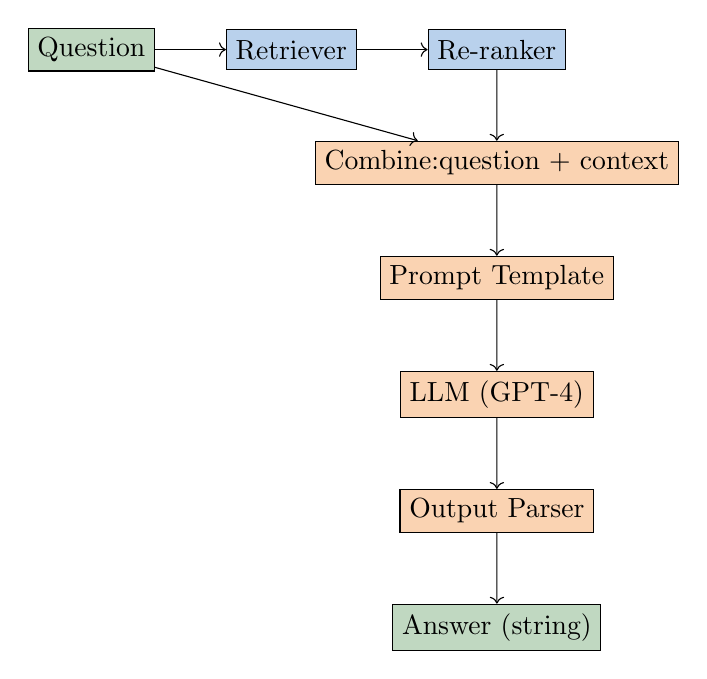
\begin{tikzpicture}[node distance=0.9cm, auto, minimum height=0.5cm, scale=0.8]
      % Input
      \node[rectangle, draw, fill=lcgreen!30] (input) {Question};

      % Parallel branches
      \node[rectangle, draw, fill=lcblue!30, right=of input] (retriever) {Retriever};
      \node[rectangle, draw, fill=lcblue!30, right=of retriever] (rerank) {Re-ranker};

      % Combine
      \node[rectangle, draw, fill=lcorange!30, below=of rerank] (combine) {Combine:\\question + context};

      % Prompt
      \node[rectangle, draw, fill=lcorange!30, below=of combine] (prompt) {Prompt Template};

      % LLM
      \node[rectangle, draw, fill=lcorange!30, below=of prompt] (llm) {LLM (GPT-4)};

      % Parser
      \node[rectangle, draw, fill=lcorange!30, below=of llm] (parser) {Output Parser};

      % Output
      \node[rectangle, draw, fill=lcgreen!30, below=of parser] (output) {Answer (string)};

      % Arrows
      \draw[->] (input) -- (retriever);
      \draw[->] (retriever) -- (rerank);
      \draw[->] (input) -- (combine);
      \draw[->] (rerank) -- (combine);
      \draw[->] (combine) -- (prompt);
      \draw[->] (prompt) -- (llm);
      \draw[->] (llm) -- (parser);
      \draw[->] (parser) -- (output);
    \end{tikzpicture}
  \end{center}

  \vspace{0.12em}
  \small Data flows top-to-bottom; parallel stages (retriever + re-rank) combine before prompt.
\end{frame}

\begin{frame}{LCEL vs Legacy Chain Classes}
  \small
  \begin{tabular}{|l|l|l|}
    \hline
    \textbf{Aspect} & \textbf{LCEL (Runnable)} & \textbf{Legacy Chain} \\
    \hline
    \textbf{Composition} & \texttt{a | b} & Chain subclassing \\
    \hline
    \textbf{Interface} & invoke, batch, stream & run, call, apply \\
    \hline
    \textbf{Async} & First-class & Bolted-on \\
    \hline
    \textbf{Streaming} & Built-in & Inconsistent \\
    \hline
    \textbf{Type safety} & Schemas & Weak \\
    \hline
    \textbf{Debugging} & Easy & Hard \\
    \hline
    \textbf{Learning curve} & Low & Medium \\
    \hline
    \textbf{Performance} & Optimized & Baseline \\
    \hline
  \end{tabular}

  \vspace{0.3em}
  \textbf{Bottom line:} Use LCEL for all new work. Legacy chains are deprecated.
\end{frame}

\begin{frame}[fragile]{Migration Example: Legacy to LCEL}
  \begin{codebox}[Before (Legacy)]
\begin{lstlisting}
from langchain.chains import LLMChain

chain = LLMChain(
    llm=model,
    prompt=prompt,
    output_parser=parser,
    verbose=True
)
result = chain.run(topic="AI")
\end{lstlisting}
  \end{codebox}

  \begin{codebox}[After (LCEL)]
\begin{lstlisting}
# Simpler, composable, type-safe
chain = prompt | model | parser
result = chain.invoke({"topic": "AI"})
\end{lstlisting}
  \end{codebox}

  \vspace{0.12em}
  \small The LCEL version is shorter, more flexible, and works with streaming, async, and batching out-of-the-box.
\end{frame}

% =============================================================================
% SECTION 10: SUMMARY & CHEAT SHEET
% =============================================================================
\section{Summary \& Cheat Sheet}

\begin{frame}{Key Takeaways}
  \begin{enumerate}\setlength{\itemsep}{1pt}
    \item \textbf{LCEL is the composition language} for LangChain — use for all new applications
    \item \textbf{Runnable protocol} is universal — invoke, batch, stream, + async variants
    \item \textbf{Pipe operator} | makes chains readable and composable
    \item \textbf{Dict syntax} creates parallel branches; RunnableBranch adds conditionals
    \item \textbf{RunnableLambda, Passthrough} give fine-grained control over data flow
    \item \textbf{Fallbacks \& retries} make chains production-ready
    \item \textbf{Batch} for throughput; stream for UX; async for scalability
    \item \textbf{Type safety} via schemas enables early error detection
    \item \textbf{LCEL scales} from simple 1-line chains to complex multi-step systems
  \end{enumerate}

  \vspace{0.3em}
  \small \textit{Philosophy: Composability over complexity. Simplicity over magic.}
\end{frame}

\begin{frame}[fragile,shrink=2]{Quick Reference}
  \small
  \begin{codebox}[Common Patterns]
\begin{lstlisting}
# Basic chain
prompt | model | parser

# Parallel (dict shorthand)
{"key": runnable1, "key2": runnable2}

# Passthrough (identity)
RunnablePassthrough()

# Lambda (wrap function)
RunnableLambda(lambda x: ...)

# Branching (conditional)
RunnableBranch((predicate, chain), default)

# Binding (partial application)
model.bind(temperature=0.1)

# Fallback (error handling)
chain.with_fallbacks([fallback1, fallback2])

# Configurable (runtime flexibility)
model.configurable_fields(...)
model.configurable_alternatives(...)

# Methods: invoke, batch, stream, ainvoke, abatch, astream
\end{lstlisting}
  \end{codebox}
\end{frame}

\begin{frame}{Self-Check Questions}
  \begin{enumerate}\setlength{\itemsep}{1pt}
    \item What is the Runnable protocol? Name all six core methods.
    \vspace{0.12em}
    \item Why use \texttt{batch()} instead of a loop of \texttt{invoke()} calls?
    \vspace{0.12em}
    \item How does the pipe operator | work? What does it create under the hood?
    \vspace{0.12em}
    \item When would you use RunnablePassthrough vs RunnableLambda?
    \vspace{0.12em}
    \item How do you add error recovery to a chain?
    \vspace{0.12em}
    \item Name three ways to make a chain configurable at runtime.
    \vspace{0.12em}
    \item What's the difference between .stream() and .batch()?
    \vspace{0.12em}
    \item How do you debug an LCEL chain to see intermediate outputs?
  \end{enumerate}
\end{frame}

\begin{frame}{Answer Key (Summary)}
  \begin{enumerate}\setlength{\itemsep}{1pt}
    \item invoke, batch, stream, ainvoke, abatch, astream
    \item \texttt{batch()} uses concurrency; much faster for multiple inputs
    \item Pipe creates \texttt{RunnableSequence}; composes left-to-right
    \item Passthrough = identity; Lambda = wraps Python functions
    \item Use \texttt{.with\_fallbacks()} and \texttt{.with\_retry()}
    \item \texttt{.bind()}, \texttt{.configurable\_fields()}, \texttt{.configurable\_alternatives()}
    \item \texttt{stream()} shows tokens in real-time; \texttt{batch()} processes many in parallel
    \item Inject \texttt{RunnableLambda(print)} steps, use \texttt{.stream()}, inspect schemas
  \end{enumerate}
\end{frame}

% =============================================================================
% ADDITIONAL RESOURCES
% =============================================================================

\begin{frame}{Resources \& Further Reading}
  \begin{itemize}\setlength{\itemsep}{1pt}
    \item \textbf{Official Docs:} \url{https://python.langchain.com/docs/expression_language}
    \item \textbf{GitHub:} \url{https://github.com/langchain-ai/langchain}
    \item \textbf{Runnable API:} \url{https://api.python.langchain.com/en/latest/runnables/}
    \item \textbf{LangSmith (debugging):} \url{https://smith.langchain.com/}
  \end{itemize}

  \vspace{0.3em}
  \textbf{Next steps:}
  \begin{itemize}\setlength{\itemsep}{1pt}
    \item Build a simple RAG chain with LCEL
    \item Experiment with streaming in a web app
    \item Profile batch() performance vs invoke() loops
    \item Try RunnableBranch for multi-path routing
    \item Explore callbacks for observability
  \end{itemize}

  \vspace{0.3em}
  \small \textit{Version: LangChain v1.2.x (March 2026)}
\end{frame}

\begin{frame}
  \centering
  \Large \textbf{Questions?}

  \vspace{2em}
  \normalsize
  Deep-dive conversation ready to continue on:
  \begin{itemize}\setlength{\itemsep}{1pt}
    \item Advanced streaming patterns
    \item Custom Runnable implementations
    \item Performance tuning for production
    \item Integration with tools, agents, memory
  \end{itemize}
\end{frame}

\end{document}
